\newpage
\section{Recommendations for further work}

This project has reached interesting results, but it can still be developed in several ways. Due to not having enough time, some ideas were only proposed and they could not be developed. They have been listed here below as an outline for those teams who agreed with us in seeing their potential related to the introduced model.
\\
\\
a) {\bf Particularization}: general findings are useful to know how to face a problem initially, but with concrete findings more adequate solutions will be found. Specific conclusions and maps for different cities and regions could be calculated.
\\
\\
b) {\bf Clustering and/or filtering antennas}: by traffic (using the 1st dataset), by location (city/field, latitude), etc.
\\
\\
c) {\bf Replicating the model and results with the 3rd dataset}.
\\
\\
d) A 60-minute time span and a daily displaying approach have been used. However, both assumptions could be modified in order to explore data from another perspective: {\bf season patterns, overlapped or shorter time spans...}
\\
\\
e) {\bf Looking for more understandable charts}: normalizing time series by dividing values by the maximum volume of the day, and some other strategies to obtain relative magnitudes.
\\
\\
f) Trying to find {\bf correlation evidence between the amount of calls rate and prosperity indicators} (business, grants, etc.).
\\
\\
g) Looking for {\bf additional socio-economic datasets} to conduct new mixed analyses (e.g. weather).
\\
\\
h) Developing a new kind of maps based on {\bf tessellations (i.e., Voronoi diagrams)}, which have been proved to be really useful for this kind of studies.
\\
\\
i) {\bf Applying DTW\footnote{http://en.wikipedia.org/wiki/Dynamic\_time\_warping} or LCS\footnote{http://en.wikipedia.org/wiki/Longest\_common\_subsequence\_problem} algorithms} to discover similarities among different traces series, in order to identify types of areas (residential, commercial, business) and to predict their evolution in mobility terms.
\\
\\
j) {\bf Trying to identify where people live and work}.
\\
\\
k) {\bf Outliers detection}: both in particular time zones and in specific regions, or also regarding patterns evolution and consolidation.
\\
\\
Moreover, some ideas and modules of this project are expected to be used into another completely different fields, so that original and novel conclusions can be reached with a high synergy value.
\\
\\
Eventually, we strongly believe that working with more detailed data (both Internet and Call/SMS communications) will allow researchers to find more accurate mathematical models and therefore, more precise and useful visualizations. Furthermore, having available longer time span datasets would assert the patterns and would  allow to describe more reliable people dynamics trends.
\\
\\
GIS tools are by themselves a fantastic way to research on geolocated data. Applying different GIS algorithms and methods could obtain new dynamics patterns, providing profitable new results to be taken into account when better development policies are decided in order to improve the people quality of life.
\\
\\
For instance, a traffic density estimation through user dynamics comunications is proposed. The next picture shows an aggregated value, however, a flow intensity related to the direction of each user trace can be applied too. A correlation of segment creation from each two antenna positions and the flow intensity between antennas taking into account the direction, could be directly applied to a real time traffic manager.

\begin{figure}[h]
\begin{center}
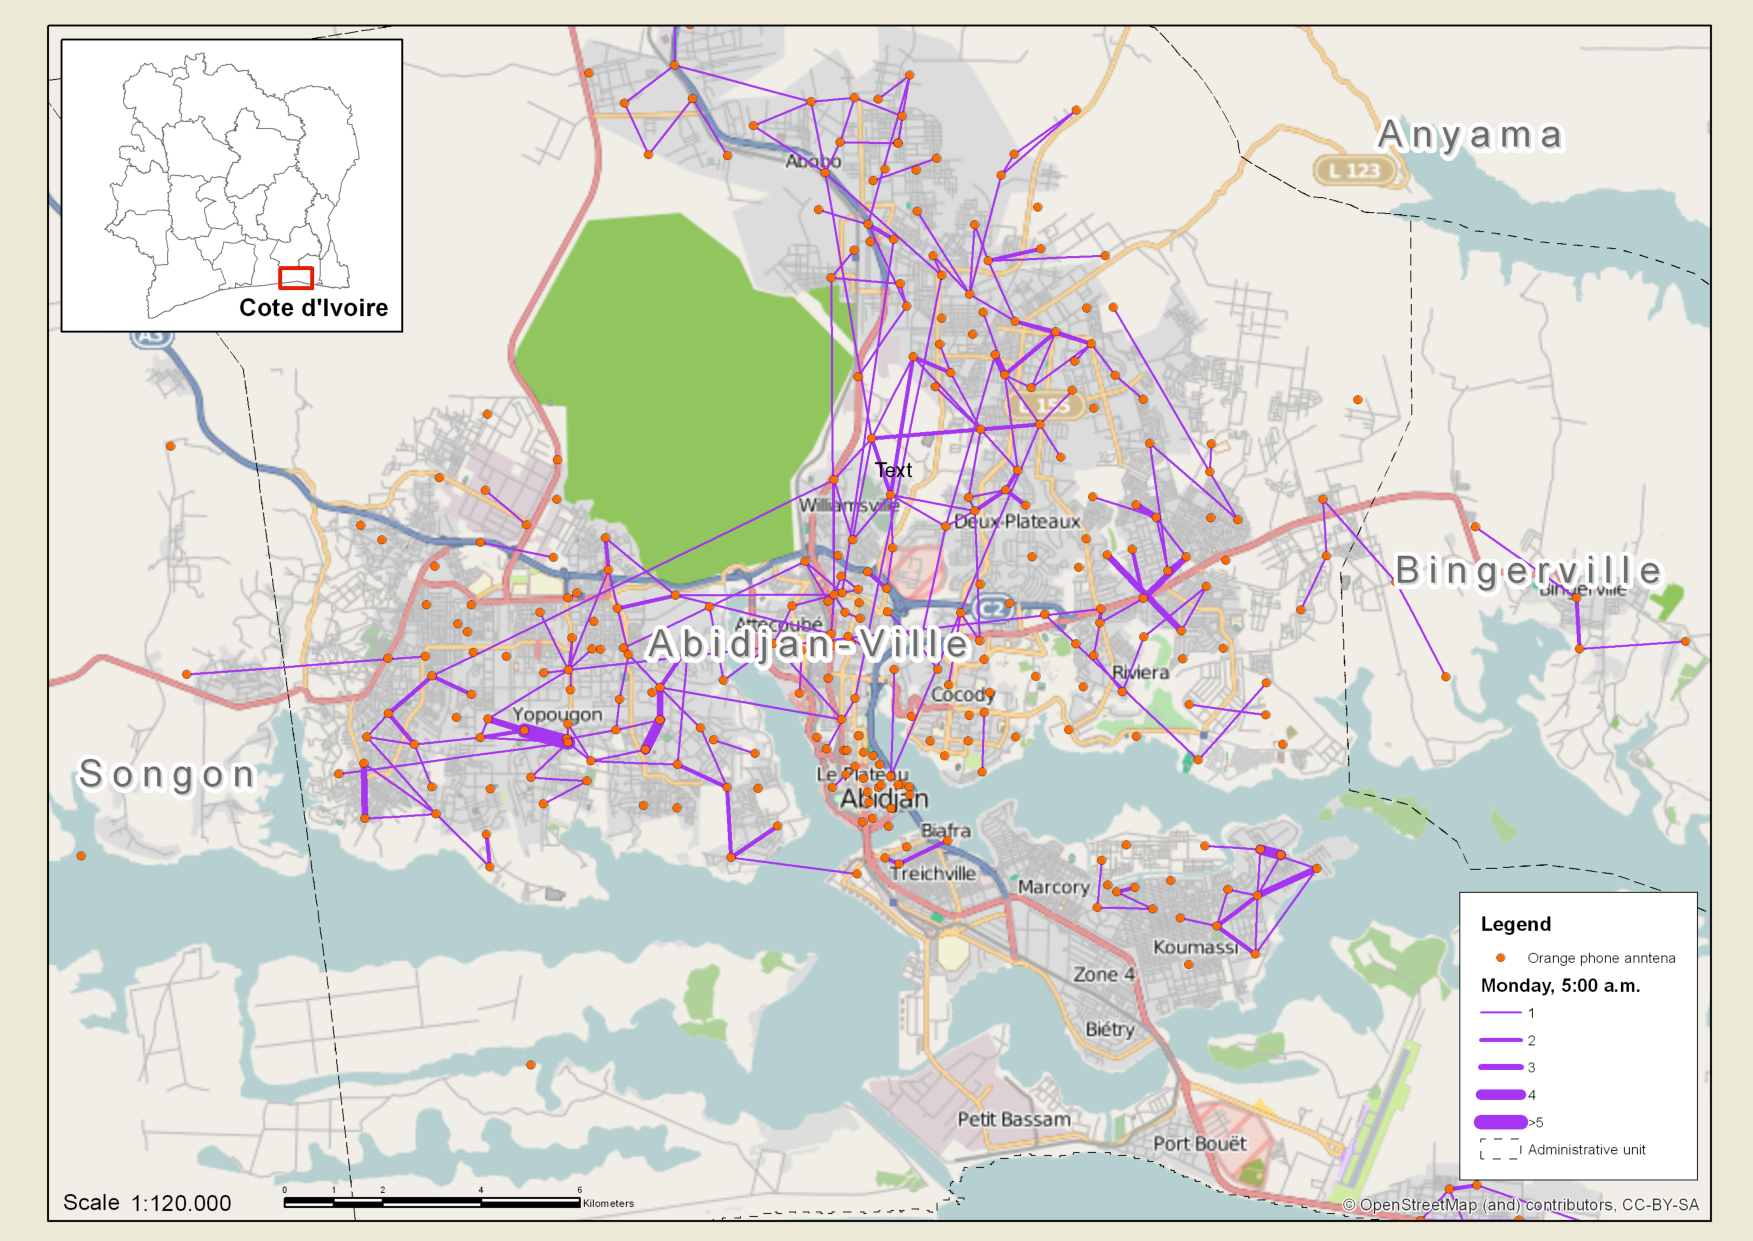
\includegraphics[scale = 0.5] {future_work/images/L_hour5_Map.pdf}
\caption{Traffic between antennas}
\label{fig:antennas_traffic}
\end{center}
\end{figure}

Starting with a file generated from the dataset that contains the geographic coordinates (longitude, latitude) of an antenna origin and those of other target antennas, together with a field that measures the traffic of information between one and the other one (‘weight’ field), we have generated the corresponding linear entities that join both positions, and the value of the calculated weight has been assigned to them. The visualization is achieved classifying the numerical field (weight) for graduated symbology using an equal interval classification method that divides the range of attribute values into five equal-sized subranges.
